\chapter{INTERFACE IMPLEMENTATION}
\label{chap:GUI_impl.tex}
The GUI provides user friendly and easy data navigation which will reduce debug efforts. All relevant processor execution log information and asm test details are provided to the user through a web interface. The interface uses data visualization JavaScript features to develop graphical representation of the log information. Features of the GUI are designed such that, traversing through the log information and comparison with the asm list file lines are made easy.  Major processor operations are categorized and extracted to have a clear view of processor actions.  From analysis done in Chapter 3, the following sets of features are expected to help the user and are our main design objective while implementing the interface:
\begin{itemize}

\item[-] Visualizing the processor execution flow in each thread
\item[-] Information regarding each Memory write/read, I/O write/read, Branching etc
\item[-] Interrupt and exception happening during execution
\item[-] Easy traversal to the asm instruction line.
\item[-] Register values at each instances
\item[-] Comparison of register values between two cycles
\item[-] All the cycle information provided by the cycle in execution log for detailed reference.
\end{itemize}
Once the simulation is completed and failure is reported the debug phase starts. This is where the role of GUI comes. From the vast information provided by the logs and test files, interfaces have to capture and represent relevant information to the user. The following section details the implementation and features of the proposed GUI. 

\section {INTERFACE IMPLEMENTATION}
GUI is implemented as a HTML web page. Each test case will have its one set of log files and asm list files. The interfaces implementation starts by taking these files are input.  Two programming languages are used for implementation:
\begin{itemize}
\item[-] Python Script for data extraction and correlating related information.
\item[-] JavaScript for designing the interface features and user interaction.
\end{itemize}
Figure x shows the implementation of GUI.

\addtocontents{toc}{\protect\setcounter{tocdepth}{2}}
%\figurename{} 
\begin{figure}[H]
\centering
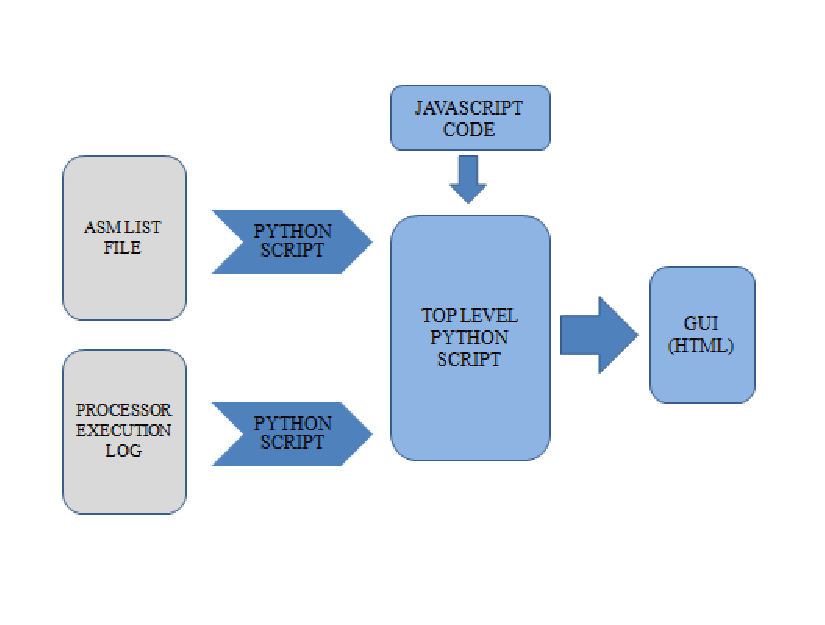
\includegraphics[width=5.5in]{./figures/gui_impl.eps}
\caption{GUI Implementation} 
\label{fig:gui_impl.eps}
\end{figure}

 Major implementation steps
\begin{itemize}
\item[-] The asm list file and processor execution file informations are extracted by python script.
\item[-] A top level python program will manipulate these information are convert it to JavaScript objects. 
\item[-] JavaScript code for developing user interactive features is written.
\item[-] The top level python program will combine the data extracted and javascriot code and generate a single HTML page. 
\end{itemize}
Inputs to the implementation are Execution log file and Asm list files. To develop the GUI the user has to execute the top level python script with these two files as input argument. The script will generate an output file which is the interface web page. Major processes involved in implementation are detailed below. 


\subsection {EXTRACTING ASM FILE INFORMATION}
The test code is written in x-86 assembly language. While debugging the instructions and values in the asm file is the expected action or value.  Each cycle in processor execution log corresponds to a particular code line in asm. However the asm code written by the verification engineer is the unscheduled code without any memory address details. For cycle comparison with execution log, the asm test file is complied first.  This is done by an assembler. Figure x shows how an asm test file is converted to a list file which hold an expanded, loop unrolled, scheduled code with memory details included.  
%\figurename{} 
%\figurename{} 
\begin{figure}[H]
\centering
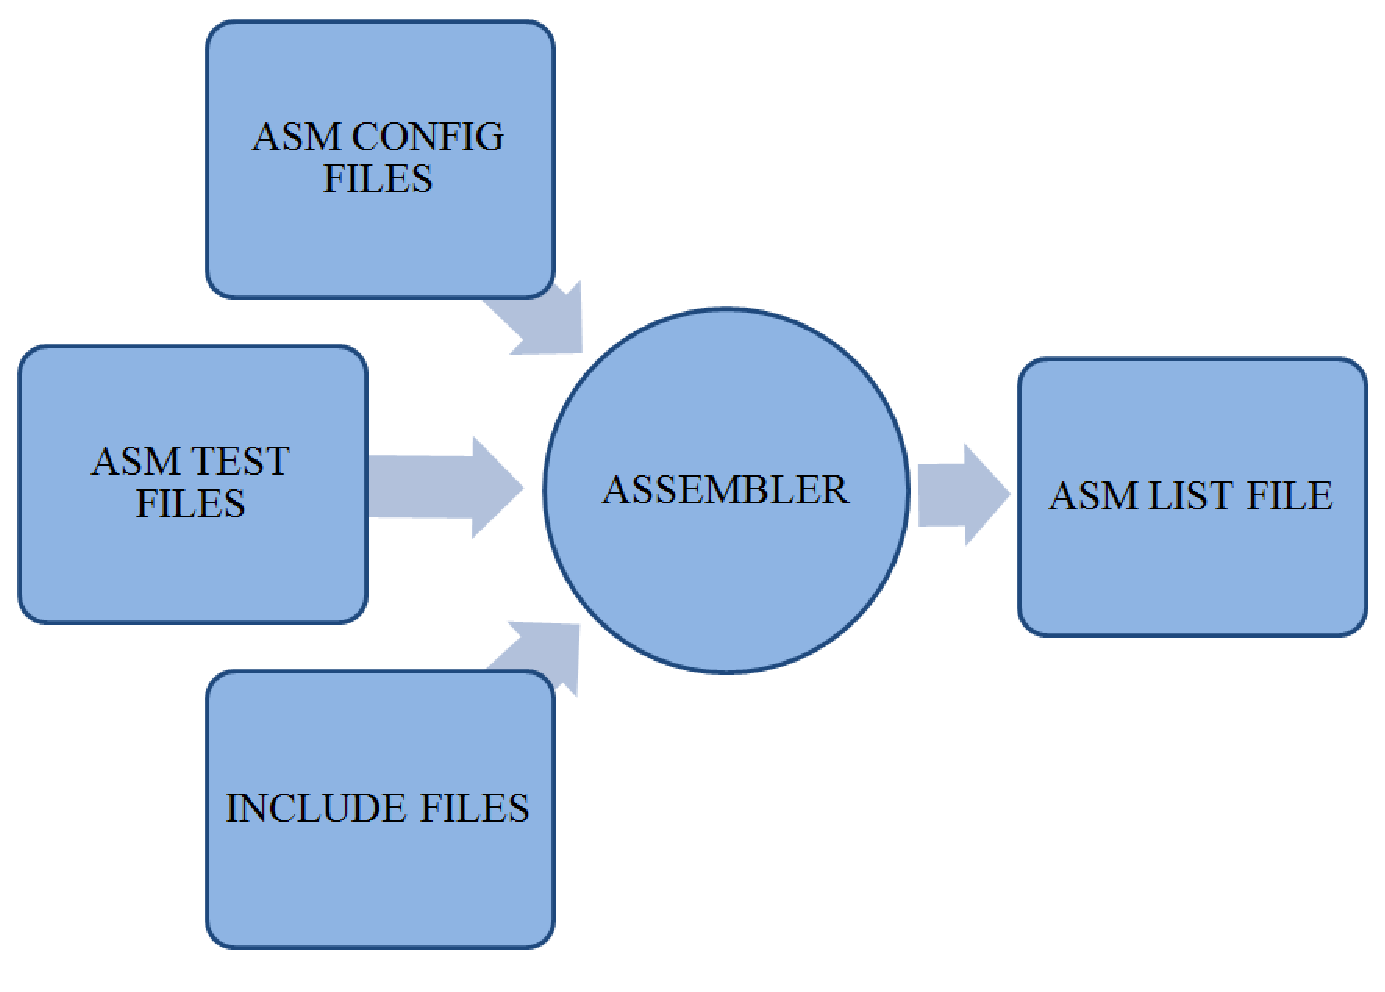
\includegraphics[width=3.5in]{./figures/asm.eps}
\caption{Assembler}
\end{figure}


A 64-bit assembler assembles asm test file, configuration file (that define the random operands, segmentation, gdt, ldt, page tables, etc,) and the include files together to generate an assembly list file [1].
\begin{figure}[H]
\centering
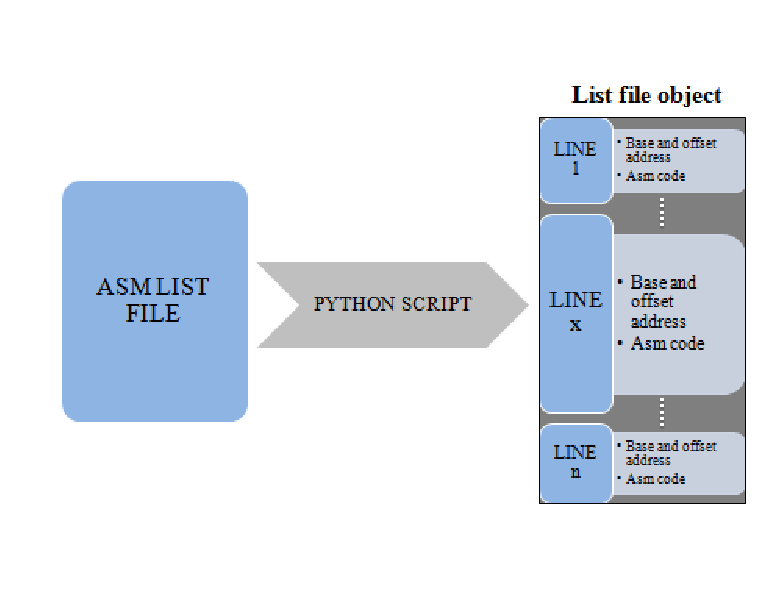
\includegraphics[width=4.5in]{./figures/list.eps}
\caption{Asm List File Extraction}
\end{figure}
List file holds details of instructions; opcodes and operand, linear address, module/register configuration details etc. For the purpose of correlating informations, a python script will extract relevant information corresponding to each instruction line in the list file.  For each line number the script will create an object which will have the following parameters.
\begin{itemize}
	\item[-] Base and offset address value
	\item[-] Instruction line number
	\item[-] The assembly code
\end{itemize}

Figure x shows how python script will read the input asm list file and generate a data structure of list objects corresponding to each line. 

\subsection {EXTRACTING EXECUTION LOG INFORMATION}
The second input to the implementation is the execution log file. As explained in previous chapters, debugging require detail traversal through this log file as it holds instruction by instruction execution details which include register states, thread details, flags information etc and other data which help in tracing out the cause of failure. 

All details given in the log file in reference to each cycle are to be extracted. The python code will extract this as well are generate a data base of log file object corresponding to each cycle of execution. These are classes with properties corresponding to major operations and register values. Each thread will have a separate handle with objects corresponding to each cycle of operation in that thread. Figure x shows how the script will read the input execution log file and generate log file objects.
Each object in the log file will have the following properties associated with it:

\begin{itemize}
 \item[-] Thread number
 \item[-]  Mode of operation
 \item[-]  Cycle number
 \item[-]  Linear address
 \item[-]  Memory write, Memory read, I/O write/read, Code read
 \item[-]  Branch target (linear address)
 \item[-]  Registers updated with new value
\end{itemize}


\subsection {Correlating asm file objects and log file objects}

Once both the input files are processed, next step is correlating the asm file object and log file object. The top level python script will combine these these to in pairs based on the address mapping. As x86 architecture follows segmented memory model along with paging, address translation is required for generating the linear/physical address [2]. For each object in the generated list file class, calculate the linear address as follows:
\\
\centerline{Linear address = Base address + Offset value}
\\
For each object in the log file class, find the corresponding list file object based on the linear address value and combine the objects.


\vspace{1.5cm}

\IncMargin{1em}
\begin{algorithm}[H]
\DontPrintSemicolon
\SetKwInOut{Input}{Input}\SetKwInOut{Output}{Output} \SetKwFunction{KwFn}{CreateDataArray}

\Input{list file objects$\rightarrow listObj[]$, log file object$\rightarrow logObj[]$}
\BlankLine
Start: \;
\For {each object $list$ in listObj}{\;
		list.address = list.Base + list.Offset\;
	}
\For {each object $log$ in logObj}{\;
	set count = 0\;
	\For {each object $list$ in listObj}{\;
	 \If{$log.address == list.address$}{
		Append each $list$.property $\rightarrow$ $log$.property\; \tcp{$log$ properties are lineNo, opcode and address}\label{cmt}
		count = 1;
		break loop\;
	}
	}
	\If{count == 0}{
	assert: $"no address match"$
	}
}
End \;
\caption{Combining List and Log File Information}
\end{algorithm}\DecMargin{1em}

\vspace{1.5cm}
Now we have a set of objects that hold log details and are linked to corresponding asm file line. Once this stage is completed we have completed all the data extraction and next phase is building the interface.

\subsection {DEVELOP THE INTERFACE}

The final step is developing the interface. As the GUI is web based, layout design is done using HTML (Hyper Text Markup Language). However for providing interactive features to the user a much more powerful language is need along with HTML and we use JavaScript.

\emph {\bf JavaScript (JS)} is an interpreted computer programming language. It is  implemented as part of web browsers so that client-side scripts could interact with the user, control the browser, communicate asynchronously, and alter the document content that was displayed. It is a multi-paradigm language, supporting object-oriented, imperative, and functional programming styles.

In addition a style sheet language called CSS (Cascading Style Sheets) is used for describing the presentation semantics (the look and formatting) of the interface page written in HTML.
%\figurename{} 
%\figurename{} 
\begin{figure}[H]
\centering
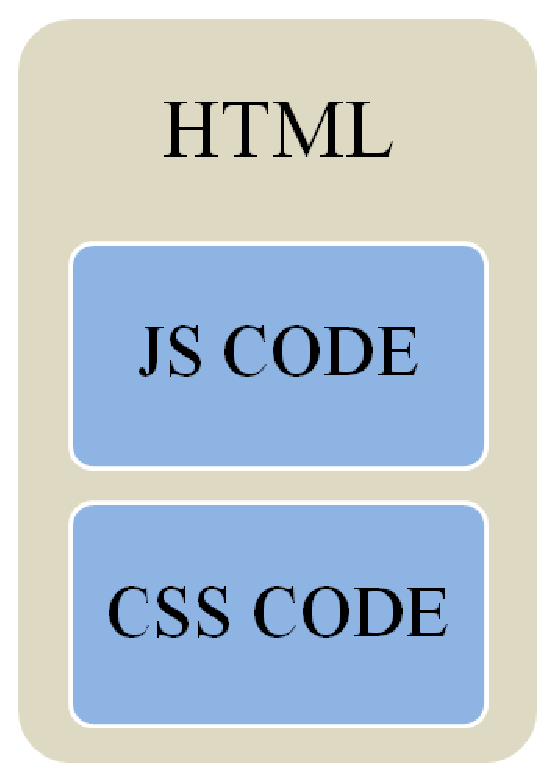
\includegraphics[width=3.5in]{./figures/html.eps}
\caption{Web Page Generation}
\end{figure}


The JavScript program and the style sheet will we embedded inside the HTML code. This connection is done by the top level python script. Figure x shows the schematic of how the files are combined with the data.



\subsubsection{CREATING JS OBJECTS}
All the dynamic features of the interface is handled by JS script. The data input to the JS is the extracted information from log files andlist files. The top level python script will convert the extracted objects into JS data array "$dataArray[]$" ; where each array element coresponds to an active thread. Active threads refer to active core or processor in a multiprocessor system.  

\IncMargin{1em}
\begin{algorithm}[H]
\DontPrintSemicolon
\SetKwInOut{Input}{Input}\SetKwInOut{Output}{Output} \SetKwFunction{KwFn}{CreateDataArray}
\KwFn {}
\BlankLine
\Begin{
\For {i in activeThreads}{\;
		\For {$log$ in logObj}{\;
		\If{log.Id == i}{
		Append $log \rightarrow	DataArray[i]$\;
		}
}
}
}
\caption{Creating JavaScript Object}
\end{algorithm}\DecMargin{1em}



Once the extracted information is converted to JS compatiable data, the interface features can utilize this. The layout for various GUI features called windows, are designed using HTML and CSS code. All the dynamic interactive featurers are handled by the JS script embedded in the final HTML web page. The following section introduces the differend windows developed for the GUI.

\section {GUI FEATURES}

\subsection {EXECUTION FLOW GRAPH}
Main feature of the web page is the graph showing the execution flow of the code. Here asm list file line numbers are plotted against the cycle during which it is executed. All the active threads have different graphs which are tabbed. Hovering the mouse over any point on the graph will display x and y axis values. 
 
This zoom enabled data graphs also provides onclick selection of specific operations e.g: Branching, Memory Write, Memory Read, Code Read etc, which will display the instances of selected operation. Each operation is distinguished by its color.   

\subsubsection {Implementation}

For the developement of execution graph we are using Dygraph JavaScript Visualization Library []. This will provide inbuild functions that enable zooming, x-y axis value display and point onClick call backs. onClick CallBack() function is called when ever a point on Dygraph is clicke and this function actives many other window.

For building the graph, input to the Dygraph is independent axis values followed by depended axis values. For each thread, a different graph is generated. The x-axis is cycle number and y-axis is the list file line number. Algorithm x explains hw the graph is build.

\IncMargin{1em}
\begin{algorithm}[H]
\DontPrintSemicolon
\SetKwInOut{Input}{Input}\SetKwInOut{Output}{Output} \SetKwFunction{KwFn}{CreateGraph}
\KwFn{}
\BlankLine
\Begin{
\For {each i in activeThread}{\;
\For {each element in dataArray[i]}{\;
	Dygraph[i] $\leftarrow [element.cycleNo , element.lineNo]$\;
	}
}
}
\caption{Creating Execution Graph}
\end{algorithm}\DecMargin{1em}

\section {REGISTER WATCH WINDOW}

Register window capture and display updated register values at a specific instance. Each thread holds its own copy of registers/flags. A selection of point on the execution flow graph will update the register window with values at that instant in the selected thread. Values of following registers and flags are provided to the user:
\begin{itemize}
	\item[-] 64 bit general purpose registers (RAX, RBX, RCX etc)
	\item[-] RFLAG (64 bit)
	\item[-] Instruction Pointer (RIP)
	\item[-] Stack Pointer (RSP)
\end{itemize}

Another feature provided by register window is comparison between register values at two different instances that is between a reference point set by Set Marker button and current selection. 

\subsubsection{Implementation}

This window is activated by the point onClick CallBack function evoked when a point is clicked on Dygraph. The function will update the register window rows set by the HTML code eg. regRow[RFLAG], regRow[RBX] etc. Also there will be a comparison with the reference point set. 

\IncMargin{1em}
\begin{algorithm}[H]
\DontPrintSemicolon
\SetKwInOut{Input}{Input}\SetKwInOut{Output}{Output} \SetKwFunction{KwFn}{pointonClickCallBack}
\KwFn{element}
\BlankLine
\Begin{
\For {each reg in RegisterSet}{
regRow$[reg]$ $\leftarrow$ element.$[reg]$ \;
	\If{(element.$[reg]$ != referenceRow.$[reg]$)}{\;
		$Highlight  regRow $ \;
	}
}
}
\caption{Creating Register Window}
\end{algorithm}\DecMargin{1em}

\subsection {INSTRUCTION WINDOW}

Instruction window give the asm file lines. A selection in execution graph will be reflected in this window by highlighting the asm file instruction corresponding to the selected point. Also the context of the selected line that is its preceding and succeeding instructions are also available in this window.
\subsubsection{Implementation}

This window is also activated by the onClick CallBack function evoked when a point is clicked on Dygraph. The function will update the instruction window set by the HTML code.

\IncMargin{1em}
\begin{algorithm}[H]
\DontPrintSemicolon
\SetKwInOut{Input}{Input}\SetKwInOut{Output}{Output} \SetKwFunction{KwFn}{onClickCallBack}
\KwFn{element}{;\
\BlankLine
\Begin{
\For {each item from elemnt-50 to element+50}{\;
	Add $item.opcode \rightarrow$ InstructionWindow\;
	}

Add $item.logInfo \rightarrow$ ExecutionLogWindow\;
}
}
\caption{Creating Instruction and Execution Log Window}
\end{algorithm}\DecMargin{1em}

\subsection {EXECUTION LOG WINDOW}

In addition to the instruction and register information, all the processor execution log information regarding the selected
instruction is also provided through execution log window.  This collected information is stored as a log file object propert "{\emph logInfo}". 

Implementation of Execution log window is given in algorithm x along with instruction window.

\subsection{SET AND CLEAR MARKER}
These two options allow setting or removing a reference point with which current register values are compared against.

\subsubsection{Implementation}

Set and Clear buttons are set using HTML form options. These elements have onClick call backs. On clicking Setbutton call back will set add values to reference register section and on click clear will remove the values in reference section.



